\documentclass{article}
\usepackage[a4paper, total={6.5in, 9in}]{geometry}
\usepackage[brazil,portuges]{babel}
\usepackage[utf8]{inputenc}
\usepackage[T1]{fontenc}
\usepackage{lmodern}
\usepackage{amsmath}
\usepackage{indentfirst}
\usepackage{titlesec}
\usepackage{todonotes}
\usepackage{enumitem}
\usepackage{tikz}
\usepackage{amsmath}
\usepackage{amsfonts}
\usepackage{amssymb}
\usepackage{gensymb}
\usepackage{array}
\usepackage{amsmath}
\usepackage{indentfirst}
\usepackage{titlesec}
\usepackage{todonotes}
\usepackage{enumitem}
\usepackage{tikz}
\usepackage{array}
\usepackage{listings}% http://ctan.org/pkg/listings
\lstset{
	basicstyle=\ttfamily,
	mathescape
}

\title{CG - Lista de Exercícios 1}
\author{André L. Mendes Fakhoury}
\date{2021}

\begin{document}

\maketitle

Nascimento: Dia $17$, Mês $4$


\section{O que são e por qual motivo utilizar coordenadas homogêneas para especificar transformações geométricas em CG?}

Coordenadas homogêneas são um sistema de coordenadas utilizadas em geometria projetiva. Nela, os pontos N-dimensionais são representados como (N+1)-dimensionais - por exemplo, um ponto no $\mathbb{R}^2$ é representado por três dimensões $(X, Y, h)$, em que $h$ é denominado parâmetro homogêneo e $x = X/h, y=Y/h$ (normalmente, em CG, utiliza-se $h = 1$). São utilizadas em CG pois as transformações geométricas podem ser representadas com mais facilidades, e um conjunto de transformações pode ser visto como multiplicações de matrizes.

\section{Apresente a matriz que representa uma transformação consistindo de uma translação seguida de uma rotação}

Fazendo uma translação $2D$ de $t_x, t_y$ e rotação de ângulo $\theta$, temos que a matriz de transformação $M$:

$$M = \underbrace{
	\begin{pmatrix}
		\cos\theta & -\sin\theta & 0\\
		\sin\theta & \cos\theta & 0\\
		0 & 0 & 1
	\end{pmatrix}
}_\text{rotação}
\cdot
\underbrace{\begin{pmatrix}
		1 & 0 & t_x\\
		0 & 1 & t_y\\
		0 & 0 & 1
\end{pmatrix}}_\text{translação}
=
\begin{pmatrix}
	\cos\theta & -\sin\theta & \cos\theta \cdot t_x - \sin\theta \cdot t_y\\
	\sin\theta & \cos\theta & \sin\theta \cdot t_x + \cos\theta \cdot t_y\\
	0 & 0 & 1
\end{pmatrix}
$$


\section{Apresenta a matriz que representa uma transformação consistindo de uma translação $t_x = M$ e $t_y = D$, seguida de uma escala uniforme $s = 2$}


$$M = \underbrace{
	\begin{pmatrix}
		2 & 0 & 0\\
		0 & 2 & 0\\
		0 & 0 & 1
	\end{pmatrix}
}_\text{escala}
\cdot
\underbrace{\begin{pmatrix}
		1 & 0 & 4\\
		0 & 1 & 17\\
		0 & 0 & 1
\end{pmatrix}}_\text{translação}
=
\begin{pmatrix}
	2 & 0 & 8\\
	0 & 2 & 34\\
	0 & 0 & 1
\end{pmatrix}
$$

\section{Verifique se $R(M+D)$ irá obter a mesma matriz de transformação do que $R(M)*R(D)$}

Calculando inicialmente $R(M + D) = R(21)$

$$\begin{pmatrix}
\cos{(21)} & -\sin{(21)} & 0\\
\sin{(21)} & \cos{(21)} & 0\\
0 & 0 & 1
\end{pmatrix}
$$

Agora a multiplicação $R(4) * R(17)$:

$$\begin{pmatrix}
	\cos{(4)} & -\sin{(4)} & 0\\
	\sin{(4)} & \cos{(4)} & 0\\
	0 & 0 & 1
\end{pmatrix} \cdot \begin{pmatrix}
\cos{(17)} & -\sin{(17)} & 0\\
\sin{(17)} & \cos{(17)} & 0\\
0 & 0 & 1
\end{pmatrix} =
$$

$$\begin{pmatrix}
	\cos{(4)} \cos{(17)} - \sin{(4)} \sin{(17)} & -\cos{(4)} \sin{(17)} - \sin{(4)} \cos{(17)} & 0\\
	\sin{(4)} \cos{(17)} + \cos{(4)} \sin{(17)} & \cos{(4)} \cos{(17)} - \sin{(4)} \sin{(17)} & 0\\
	0 & 0 & 1
\end{pmatrix}$$

\noindent e, como $\cos{(a + b)} = \cos{(a)} \cos{(b)} - \sin{(a)} \sin{(b)}$ e $\sin{(a + b)} = \sin{(a)} \cos{(b)} + \sin{(b)} \cos{(a)}$, vemos que as duas matrizes são equivalentes.

\section{Forneça a matriz de transformação que realiza a transformação abaixo (a seta indica o objeto inicial e o final após a transformação). Em seguida, apresente as coordenadas do objeto para uma escala uniforme $s = M$.}

\begin{figure}[ht!]
	\centering
	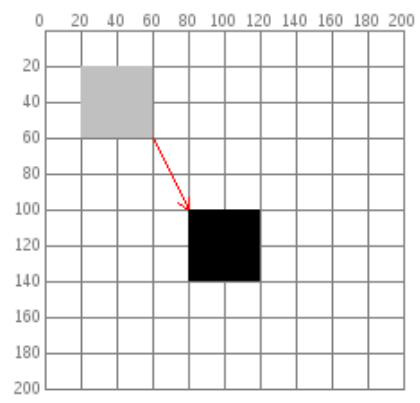
\includegraphics[width=0.5\textwidth]{img/img1.png}
\end{figure}

A figura indica uma translação de $t_x = 60, t_y = 80$. Pode ser indicada pela matriz:

$$M = \begin{pmatrix}
	1 & 0 & 60\\
	0 & 1 & 80\\
	0 & 0 & 1
\end{pmatrix}$$

As coordenadas do objeto podem ser representadas pelo quadrado $ABCD = (A=(80, 100), B=(120, 100), C=(120, 140), D=(80, 140))$. As coordenadas do objeto após uma escala uniforme $s = 4$ serão:

$$A' = \begin{bmatrix}
	x'\\
	y'\\
	1
\end{bmatrix} = \begin{bmatrix}
	4 & 0 & 0\\
	0 & 4 & 0\\
	0 & 0 & 1
\end{bmatrix} \cdot \begin{bmatrix}
	80\\
	100\\
	1
\end{bmatrix} = \begin{bmatrix}
	360\\
	400\\
	1
\end{bmatrix}$$

$$B' = \begin{bmatrix}
	x'\\
	y'\\
	1
\end{bmatrix} = \begin{bmatrix}
	4 & 0 & 0\\
	0 & 4 & 0\\
	0 & 0 & 1
\end{bmatrix} \cdot \begin{bmatrix}
	120\\
	100\\
	1
\end{bmatrix} = \begin{bmatrix}
	480\\
	400\\
	1
\end{bmatrix}$$

$$C' = \begin{bmatrix}
	x'\\
	y'\\
	1
\end{bmatrix} = \begin{bmatrix}
	4 & 0 & 0\\
	0 & 4 & 0\\
	0 & 0 & 1
\end{bmatrix} \cdot \begin{bmatrix}
	120\\
	140\\
	1
\end{bmatrix} = \begin{bmatrix}
	480\\
	560\\
	1
\end{bmatrix}$$

$$D' = \begin{bmatrix}
	x'\\
	y'\\
	1
\end{bmatrix} = \begin{bmatrix}
	4 & 0 & 0\\
	0 & 4 & 0\\
	0 & 0 & 1
\end{bmatrix} \cdot \begin{bmatrix}
	80\\
	140\\
	1
\end{bmatrix} = \begin{bmatrix}
	360\\
	560\\
	1
\end{bmatrix}$$

Portanto, as novas coordenadas do quadrado são $A'B'C'D' = (A'=(360, 400), B'=(480, 400), C'=(480, 560), D'=(360, 560)).$

\section{Abaixo é apresentada a matriz resultante de quatro transformações. Aplique esta transformação em triângulo ABC (A=(0, 0), B = (1, 0), C = (0, 1)) e mostre o resultado (novos vértices e o desenho. Em seguida, faça uma translação $t_x = M/10$ e $t_y = M / 10$.}

\begin{figure}[ht!]
	\centering
	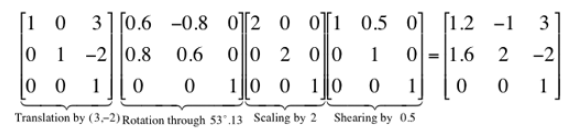
\includegraphics[width=0.8\textwidth]{img/img2.png}
\end{figure}

Calculando a transformação em cada vértice do triângulo, temos:

$$A' = \begin{bmatrix}
x'\\
y'\\
1
\end{bmatrix} = \begin{bmatrix}
1.2 & -1 & 3\\
1.6 & 2 & -2\\
0 & 0 & 1
\end{bmatrix} \cdot \begin{bmatrix}
0\\
0\\
1
\end{bmatrix} = \begin{bmatrix}
3\\
-2\\
1
\end{bmatrix}$$

$$B' = \begin{bmatrix}
	x'\\
	y'\\
	1
\end{bmatrix} = \begin{bmatrix}
	1.2 & -1 & 3\\
	1.6 & 2 & -2\\
	0 & 0 & 1
\end{bmatrix} \cdot \begin{bmatrix}
	1\\
	0\\
	1
\end{bmatrix} = \begin{bmatrix}
	4.2\\
	-0.4\\
	1
\end{bmatrix}$$

$$C' = \begin{bmatrix}
	x'\\
	y'\\
	1
\end{bmatrix} = \begin{bmatrix}
	1.2 & -1 & 3\\
	1.6 & 2 & -2\\
	0 & 0 & 1
\end{bmatrix} \cdot \begin{bmatrix}
	0\\
	1\\
	1
\end{bmatrix} = \begin{bmatrix}
	2\\
	0\\
	1
\end{bmatrix}$$

Portanto, o novo triângulo tem vértices $(A'=(3, -2), B'=(4.2, -0.4), C'=(2, 0))$:

\begin{figure}[ht!]
	\centering
	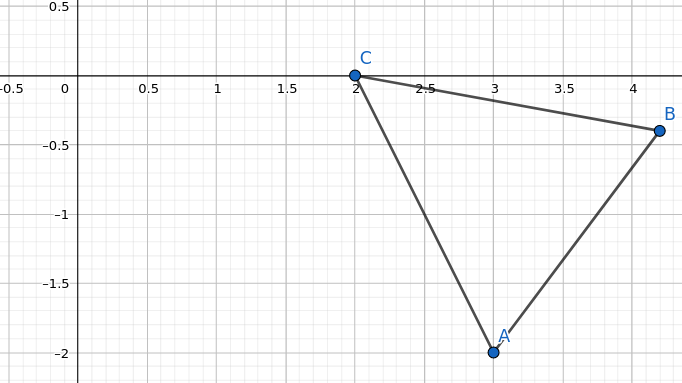
\includegraphics[width=0.5\textwidth]{img/n_triangle.png}
\end{figure}

Fazendo uma translação $t_x = 0.4, t_y = 0.4$, temos:

$$A'' = \begin{bmatrix}
	x''\\
	y''\\
	1
\end{bmatrix} = \begin{bmatrix}
	1 & 0 & 0.4\\
	0 & 1 & 0.4\\
	0 & 0 & 1
\end{bmatrix} \cdot \begin{bmatrix}
	3\\
	-2\\
	1
\end{bmatrix} = \begin{bmatrix}
	3.4\\
	-1.6\\
	1
\end{bmatrix}$$


$$B'' = \begin{bmatrix}
	x''\\
	y''\\
	1
\end{bmatrix} = \begin{bmatrix}
	1 & 0 & 0.4\\
	0 & 1 & 0.4\\
	0 & 0 & 1
\end{bmatrix} \cdot \begin{bmatrix}
	4.2\\
	-0.4\\
	1
\end{bmatrix} = \begin{bmatrix}
	4.6\\
	0\\
	1
\end{bmatrix}$$

$$C'' = \begin{bmatrix}
	x''\\
	y''\\
	1
\end{bmatrix} = \begin{bmatrix}
	1 & 0 & 0.4\\
	0 & 1 & 0.4\\
	0 & 0 & 1
\end{bmatrix} \cdot \begin{bmatrix}
	2\\
	0\\
	1
\end{bmatrix} = \begin{bmatrix}
	2.4\\
	0.4\\
	1
\end{bmatrix}$$

Portanto, os novos vértices serão $(A''=(3.4, -1.6), B''=(4.6, 0), C''=(2.4, 0.4))$.

\section{Mostre que a ordem das transformações pode modificar a matriz de transformação resultante (problema da comutatividade). OBS: É suficiente fornecer um exemplo.}

Um possível exemplo não comutativo é a transformação de translação em conjunto com escala (escala constante $s_x = s_y = s$). Seja $M_1$ a matriz resultante de uma escala seguida de translação e $M_2$ a matriz resultante de uma translação seguida de escala:

$$M_1 = \begin{pmatrix}
		1 & 0 & t_x\\
		0 & 1 & t_y\\
		0 & 0 & 1
\end{pmatrix}
\cdot
	\begin{pmatrix}
		s & 0 & 0\\
		0 & s & 0\\
		0 & 0 & 1
	\end{pmatrix}
=
\begin{pmatrix}
	s & 0 & t_x\\
	0 & s & t_y\\
	0 & 0 & 1
\end{pmatrix}
$$

$$M_2 = \begin{pmatrix}
	s & 0 & 0\\
	0 & s & 0\\
	0 & 0 & 1
\end{pmatrix}
\cdot
\begin{pmatrix}
	1 & 0 & t_x\\
	0 & 1 & t_y\\
	0 & 0 & 1
\end{pmatrix}
=
\begin{pmatrix}
	s & 0 & s \cdot t_x\\
	0 & s & s \cdot t_y\\
	0 & 0 & 1
\end{pmatrix}
$$

Como $M_1 \neq M_2$, as transformações não são comutativas.

\section{As transformações de rotação e escala são comutativas entre si?}

Seja $M_1$ a matriz resultante de uma escala seguida de rotação e $M_2$ a matriz resultante de uma rotação seguida de escala:

$$M_1 = \begin{pmatrix}
	\cos\theta & -\sin\theta & 0\\
	\sin\theta & \cos\theta & 0\\
	0 & 0 & 1
\end{pmatrix} \cdot \begin{pmatrix}
s_x & 0 & 0\\
0 & s_y & 0\\
0 & 0 & 1
\end{pmatrix} = \begin{pmatrix}
\cos\theta \cdot s_x & -\sin\theta \cdot s_y & 0\\
\sin\theta \cdot s_x & \cos\theta \cdot s_y & 0\\
0 & 0 & 1
\end{pmatrix}$$

$$M_2 = \begin{pmatrix}
	s_x & 0 & 0\\
	0 & s_y & 0\\
	0 & 0 & 1
\end{pmatrix} \cdot \begin{pmatrix}
\cos\theta & -\sin\theta & 0\\
\sin\theta & \cos\theta & 0\\
0 & 0 & 1
\end{pmatrix} = \begin{pmatrix}
\cos\theta \cdot s_x & -\sin\theta \cdot s_x & 0\\
\sin\theta \cdot s_y & \cos\theta \cdot s_y & 0\\
0 & 0 & 1
\end{pmatrix}$$

Como $M_1 \neq M_2$, não são comutativas. Porém, caso a escala seja uniforme $s_x = s_y$, as transformações são comutativas, pois a matriz de transformação resultante será a mesma.

\section{As transformações de translação e escala são comutativas entre si? E entre translação e rotação?}

Já foi demonstrado no exercício $7$ que as transformações de translação e escala não são comutativas entre si: seja $M_1$ a matriz resultante de uma escala seguida de translação e $M_2$ a matriz resultante de uma translação seguida de escala:

$$M_1 = \begin{pmatrix}
	1 & 0 & t_x\\
	0 & 1 & t_y\\
	0 & 0 & 1
\end{pmatrix}
\cdot
\begin{pmatrix}
	s & 0 & 0\\
	0 & s & 0\\
	0 & 0 & 1
\end{pmatrix}
=
\begin{pmatrix}
	s & 0 & t_x\\
	0 & s & t_y\\
	0 & 0 & 1
\end{pmatrix}
$$

$$M_2 = \begin{pmatrix}
	s & 0 & 0\\
	0 & s & 0\\
	0 & 0 & 1
\end{pmatrix}
\cdot
\begin{pmatrix}
	1 & 0 & t_x\\
	0 & 1 & t_y\\
	0 & 0 & 1
\end{pmatrix}
=
\begin{pmatrix}
	s & 0 & s \cdot t_x\\
	0 & s & s \cdot t_y\\
	0 & 0 & 1
\end{pmatrix}
$$

\noindent vemos que $M_1 \neq M_2$, portanto não são comutativas.

Verifiquemos agora as transformações de translação e rotação: seja $M_1$ a matriz transformação de rotação seguida de translação e $M_2$ a matriz transformação de translação seguida de rotação:

$$M_1 = \begin{pmatrix}
		1 & 0 & t_x\\
		0 & 1 & t_y\\
		0 & 0 & 1
\end{pmatrix}
\cdot
	\begin{pmatrix}
		\cos\theta & -\sin\theta & 0\\
		\sin\theta & \cos\theta & 0\\
		0 & 0 & 1
	\end{pmatrix}
=
\begin{pmatrix}
	\cos\theta & -\sin\theta & t_x\\
	\sin\theta & \cos\theta & t_y\\
	0 & 0 & 1
\end{pmatrix}
$$

$$M_2 = \begin{pmatrix}
	\cos\theta & -\sin\theta & 0\\
	\sin\theta & \cos\theta & 0\\
	0 & 0 & 1
\end{pmatrix}
\cdot
\begin{pmatrix}
	1 & 0 & t_x\\
	0 & 1 & t_y\\
	0 & 0 & 1
\end{pmatrix}
=
\begin{pmatrix}
	\cos\theta & -\sin\theta & \cos\theta \cdot t_x -\sin\theta \cdot t_y\\
	\sin\theta & \cos\theta & \sin\theta \cdot t_x +\cos\theta \cdot t_y\\
	0 & 0 & 1
\end{pmatrix}
$$

Como $M_1 \neq M_2$, temos que a transformação de translação e rotação não são comutativas entre si.


\section{Forneça a sequência de transformações que leva o triângulo T1 ao triângulo T2 e dê a matriz resultante.}

\begin{figure}[ht!]
	\centering
	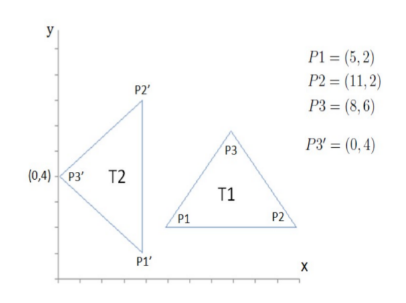
\includegraphics[width=0.5\textwidth]{img/img3.png}
\end{figure}

Uma possível sequência de transformações que pode ser aplicada é a translação $t_x = -4, t_y = -6$ seguida de uma rotação em $90 \degree$. Outra possibilidade (com um passo a mais) seria realizar anteriormente uma translação do objeto para a origem, para posterior rotação e translação para a posição descrita por $T2$.

$$M = \begin{pmatrix}
	\cos90 \degree & -\sin90 \degree & 0 & 0\\
	\sin90 \degree & \cos90 \degree & 0 & 0\\
	0 & 0 & 1 & 0\\
	0 & 0 & 0 & 1
\end{pmatrix}
\cdot
\begin{pmatrix}
	1 & 0 & 0 & -4\\
	0 & 1 & 0 & -6\\
	0 & 0 & 1 & 0\\
	0 & 0 & 0 & 1
\end{pmatrix}
=
\begin{pmatrix}
	0 & -1 & 0 & 6\\
	1 & 0 & 0 & -4\\
	0 & 0 & 1 & 0\\
	0 & 0 & 0 & 1
\end{pmatrix}
$$


\section{Seja um quadrado de lado $L = 5$, inicialmente posicionado em $x = M$ e $y = D$. Calcule e apresente a matriz de transformação que faça o quadrado rotacionar 45 graus em relação ao seu próprio centro. Apresente os vértices iniciais e finais do quadrado.}

O quadrado está posicionado com os vértices $ABCD = (A=(17, 4), B=(22, 4), C=(22, 9), D=(17, 9))$.

Para o quadrado rotacionar em torno do seu próprio centro, deve-se aplicar inicialmente uma translação para a origem, realizar a rotação e então realizar a translação de volta para a posição original. Como a origem deve receber o centro do quadrado, realiza-se as operações com relação ao ponto de referência $t_x = 19.5, t_y = 6.5$.

$$M = \begin{pmatrix}
	1 & 0 & t_x\\
	0 & 1 & t_y\\
	0 & 0 & 1
\end{pmatrix} \cdot \begin{pmatrix}
	\cos\theta & -\sin\theta & 0\\
	\sin\theta & \cos\theta & 0\\
	0 & 0 & 1
\end{pmatrix}
\cdot
\begin{pmatrix}
	1 & 0 & -t_x\\
	0 & 1 & -t_y\\
	0 & 0 & 1
\end{pmatrix} =$$

$$= \begin{pmatrix}
	\cos\theta & -\sin\theta & t_x - t_x \cdot \cos\theta + t_y \cdot \sin\theta\\
	\sin\theta & \cos\theta & t_y - t_y \cdot \cos\theta - t_x \cdot \sin\theta\\
	0 & 0 & 1
\end{pmatrix}$$

\noindent e, como $t_x = 19.5, t_y = 6.5, \theta = 45\degree$:

$$M = \begin{pmatrix}
	0.707 & -0.707 & 10.308\\
	0.707 & 0.707 & -11.885\\
	0 & 0 & 1
\end{pmatrix}$$

Aplicando em cada vértice, temos:

$$A' = \begin{bmatrix}
	x'\\
	y'\\
	1
\end{bmatrix} = \begin{bmatrix}
0.707 & -0.707 & 10.308\\
0.707 & 0.707 & -11.885\\
0 & 0 & 1
\end{bmatrix} \cdot \begin{bmatrix}
17\\
4\\
1
\end{bmatrix} = \begin{bmatrix}
19.5\\
2.964\\
1
\end{bmatrix}$$

$$B' = \begin{bmatrix}
	x'\\
	y'\\
	1
\end{bmatrix} = \begin{bmatrix}
	0.707 & -0.707 & 10.308\\
	0.707 & 0.707 & -11.885\\
	0 & 0 & 1
\end{bmatrix} \cdot \begin{bmatrix}
	22\\
	4\\
	1
\end{bmatrix} = \begin{bmatrix}
	23.036\\
	6.5\\
	1
\end{bmatrix}$$

$$C' = \begin{bmatrix}
	x'\\
	y'\\
	1
\end{bmatrix} = \begin{bmatrix}
	0.707 & -0.707 & 10.308\\
	0.707 & 0.707 & -11.885\\
	0 & 0 & 1
\end{bmatrix} \cdot \begin{bmatrix}
	22\\
	9\\
	1
\end{bmatrix} = \begin{bmatrix}
	19.5\\
	10.036\\
	1
\end{bmatrix}$$

$$D' = \begin{bmatrix}
	x'\\
	y'\\
	1
\end{bmatrix} = \begin{bmatrix}
	0.707 & -0.707 & 10.308\\
	0.707 & 0.707 & -11.885\\
	0 & 0 & 1
\end{bmatrix} \cdot \begin{bmatrix}
	17\\
	9\\
	1
\end{bmatrix} = \begin{bmatrix}
	15.964\\
	6.5\\
	1
\end{bmatrix}$$

Com isso, temos os vértices iniciais $ABCD = (A=(17, 4), B=(22, 4), C=(22, 9), D=(17, 9))$ e os vértices finais $A'B'C'D' = (A'=(19.5, 2.964), B'=(23.036, 6.5), C'=(19.5, 10.036), D'=(15.964, 6.5))$. A rotação pode ser vista na seguinte figura:

\begin{figure}[htb]
	\centering
	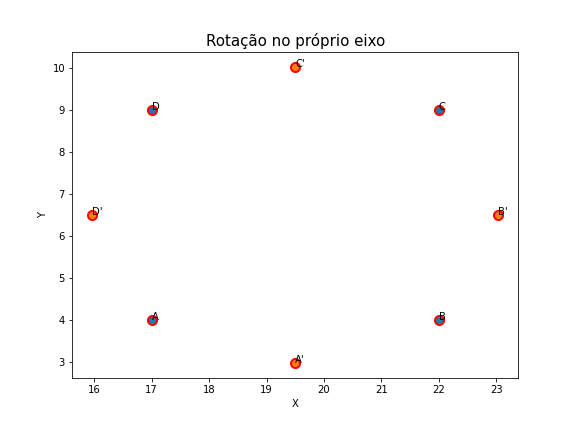
\includegraphics[width=0.7\textwidth]{img/rotation.png}
	\label{fig:rot}
\end{figure}


\section{Dado um vértice/ponto posicionado em $x = D$ e $y = M$, apresente as matrizes de transformação para (1) espelhar esse vértice em relação ao eixo X e (2) espelhar esse vértice em relação ao eixo Y.}

Seja $M_1$ a matriz transformação para espelhar em relação ao eixo X e $M_2$ a matriz transformação para espelhar em relação ao eixo Y:

$$M_1 = \begin{pmatrix}
	1 & 0 & 0\\
	0 & -1 & 0\\
	0 & 0 & 1
\end{pmatrix}$$

Ou seja, $x' = x$ e $y' = -y$. Como $(x, y) = (17, 4)$, temos que $(x', y') = (17, -4)$.


$$M_2 = \begin{pmatrix}
	-1 & 0 & 0\\
	0 & 1 & 0\\
	0 & 0 & 1
\end{pmatrix}$$


Ou seja, $x' = -x$ e $y' = y$. Como $(x, y) = (17, 4)$, temos que $(x', y') = (-17, 4)$.

\end{document}